% \begin{table*}[h!]
% \centering
% \resizebox{\textwidth}{!}{%
% {\fontsize{8}{12}\selectfont
% \begin{tabular}{lccccc|c}
% \toprule
% Model & Action Justification & Expected Action & Linguistic Habits & Persona Consistency & Toxicity Control & \textbf{\score} \\
% \midrule
% LLaMA-2-13b       & 3.96 (0.80) & 3.87 (0.84) & 3.77 (0.87) & 4.12 (0.92) & 4.18 (1.00) & 3.98 (0.49) \\
% GPT 3.5           & 4.31 (0.49) & 4.28 (0.49) & 3.63 (0.68) & 4.70 (0.41) & 4.96 (0.30) & 4.38 (0.23) \\
% LLaMA-2-70b       & 4.44 (0.55) & 4.32 (0.60) & 3.85 (0.73) & 4.67 (0.56) & 4.68 (0.77) & 4.39 (0.35) \\
% LLaMA-3-8b        & 4.55 (0.46) & 4.43 (0.49) & 3.97 (0.69) & 4.77 (0.37) & 4.74 (0.68) & 4.49 (0.27) \\
% Claude 3 Haiku    & 2.47 (1.64) & 4.28 (0.72) & 3.04 (1.01) & 3.47 (1.57) & 4.94 (0.36) & 3.64 (0.57) \\
% Claude 3.5 Sonnet & 4.52 (0.67) & \textbf{4.37} (0.60) & 3.98 (0.71) & \textbf{4.81} (0.51) & 4.88 (0.54) & \textbf{4.51} (0.37) \\
% GPT-4.1           & 4.51 (0.11) & 4.20 (0.16) & 4.10 (0.27) & 4.67 (0.11) & \textbf{4.96} (0.22) & 4.49 (0.09) \\
% Deepseek-V3          & 4.54 (0.13) & 4.20 (0.16) & \textbf{4.26} (0.21) & 4.66 (0.11) & 4.74 (0.46) & 4.48 (0.10) \\
% LLaMA-3.3-70b         & 4.34 (0.11) & 4.12 (0.17) & 3.92 (0.24) & 4.56 (0.13) & 4.86 (0.34) & 4.36 (0.09) \\
% GPT-4.5           & \textbf{4.57} (0.15) & 4.21 (0.17) & 4.14 (0.24) & 4.70 (0.12) & \textbf{4.96} (0.22) & \textbf{4.51} (0.08) \\
% \bottomrule
% \end{tabular}
% }
% }
% \caption{Benchmarked results of 10 LLMs on 200 personas descriptions and 10 questions per task totaling 10K questions. As part of \benchmark we propose 5 evaluation tasks all of which are grounded in decision theory to properly evaluate persona agents on different axes of interactions with environments. Bolded results indicate the best scoring model for each task. Standard deviations for each task and model are included within parentheses.}
% \label{tab:results}
% \end{table*}



\begin{table*}[h!]
\centering
\rowcolors{2}{rowgray}{white}  % alternating row colors
\resizebox{\textwidth}{!}{%
\begin{tabular}{l
                S[table-format=1.2(2)]
                S[table-format=1.2(2)]
                S[table-format=1.2(2)]
                S[table-format=1.2(2)]
                S[table-format=1.2(2)]
                S[table-format=1.2(2)]}
\toprule
\rowcolor{white}
\textbf{Model} & 
\textbf{Action Just.} & 
\textbf{Expected Action} & 
\textbf{Ling. Habits} & 
\textbf{Persona Cons.} & 
\textbf{Toxicity Ctrl.} & 
\textbf{\score} \\
\midrule
\textsc{LLaMA-2-13b}       & 3.96(0.80) & 3.87(0.84) & 3.77(0.87) & 4.12(0.92) & 4.18(1.00) & 3.98(0.49) \\
\textsc{GPT 3.5}           & 4.31(0.49) & 4.28(0.49) & 3.63(0.68) & 4.70(0.41) & 4.96(0.30) & 4.38(0.23) \\
\textsc{LLaMA-2-70b}       & 4.44(0.55) & 4.32(0.60) & 3.85(0.73) & 4.67(0.56) & 4.68(0.77) & 4.39(0.35) \\
\textsc{LLaMA-3-8b}        & 4.55(0.46) & 4.43(0.49) & 3.97(0.69) & 4.77(0.37) & 4.74(0.68) & 4.49(0.27) \\
\textsc{Claude 3 Haiku}    & 2.47(1.64) & 4.28(0.72) & 3.04(1.01) & 3.47(1.57) & 4.94(0.36) & 3.64(0.57) \\
% \rowcolor{highlight}
\textsc{Claude 3.5 Sonnet} & 4.52(0.67) & 4.37(0.60) & 3.98(0.71) & \bfseries 4.81(0.51) & 4.88(0.54) & \bfseries 4.51(0.37) \\
\textsc{GPT-4.1}           & 4.51(0.11) & 4.20(0.16) & 4.10(0.27) & 4.67(0.11) & \bfseries 4.96(0.22) & 4.49(0.09) \\
\textsc{Deepseek-V3}       & 4.54(0.13) & 4.20(0.16) & \bfseries 4.26(0.21) & 4.66(0.11) & 4.74(0.46) & 4.48(0.10) \\
\textsc{LLaMA-3.3-70b}     & 4.34(0.11) & 4.12(0.17) & 3.92(0.24) & 4.56(0.13) & 4.86(0.34) & 4.36(0.09) \\
% \rowcolor{highlight}
\textsc{GPT-4.5}           & \bfseries 4.57(0.15) & 4.21(0.17) & 4.14(0.24) & 4.70(0.12) & \bfseries 4.96(0.22) & \bfseries 4.51(0.08) \\
\bottomrule
\end{tabular}
}
\caption{Benchmarked results of 10 LLMs on 200 personas and 10 questions per task totaling 10K questions. Bolded results indicate the best scoring model for each task. Standard deviations for each task and model also included.}
\label{tab:results}
\end{table*}


\subsection{Experimental Settings}

\paragraph{Benchmarked Models}
Our study evaluates the proficiency of four open-source and three closed-source LLMs in acting as persona agents and interacting within seeded environments. The open-source models under examination are: \textsc{LLaMA-2-13b}, \textsc{LLaMA-2-70b}, \textsc{LLaMA-3.3-70b}, \textsc{LLaMA-3-8b}, and \textsc{Deepseek-V3}. The closed-source models include: \textsc{GPT 3.5}, \textsc{Claude 3 Haiku}, \textsc{GPT 4.1}, \textsc{GPT 4.5} and \textsc{Claude 3.5 Sonnet}.

\paragraph{Environment and Question Generation} We use \textsc{GPT-4o} (gpt-4o-2024-05-13) for: (1) selecting persona-relevant environments, (2) generating task-specific questions for each \benchmark task based on the persona and chosen settings. We set the temperature and nucleus sampling parameters to 0.9 for environment selection and question generation. We generated 200 personas using \textsc{GPT-4o} for our evaluation. We observe that beyond 200 personas, \textsc{GPT-4o}'s limited diversity became a constraining factor, leading to overlapping persona attributes that compromised overall diversity. We release our benchmark under the MIT license. Future efforts to enhance or modify our persona list should consider leveraging techniques for diversifying LLM generations \cite{zhang2024forcing}.

\paragraph{Evaluator Models} In our experiments, we employ two evaluator models to assess persona agent responses according to task-specific rubrics: \textsc{GPT-4o} and \textsc{LLaMA-3-70b}. Both evaluator models operated at 0 temperature for a mostly deterministic output.

\subsection{Main Results}

% \begin{table*}[h]
% \centering
% \resizebox{\textwidth}{!}{
% {\fontsize{9}{12}\selectfont
% \begin{tabular}{lccccc|c}
% \toprule
% Model & Action Justification & Expected Action & Linguistic Habits & Persona Consistency & Toxicity Control & \textbf{\score} \\
% \midrule
% \textsc{LLaMA-2-13b} & 83.6\% / 76.1\% & 75.6\% / 65.2\% & 84.3\% / 77.2\% & 84.6\% / 75.6\% & 68.2\% / 62.4\% & 62.9\% / 49.2\% \\
% \textsc{GPT 3.5} & 61.1\% / 58.7\% & 80.1\% / 74.0\% & 73.6\% / 63.6\% & 61.6\% / 61.0\% & 50.0\% / 49.8\% & 78.0\% / 67.4\% \\
% \textsc{LLaMA-2-70b} & 67.0\% / 61.3\% & 84.8\% / 77.1\% & 55.8\% / 48.4\% & 40.0\% / 39.2\% & 76.7\% / 72.9\% & 84.4\% / 71.6\% \\
% \bottomrule
% \end{tabular}
% }
% }
% \caption{Average correlation scores across randomly sampled 100 personas between \textsc{GPT 3.5}, \textsc{LLaMA-2-13b}, and \textsc{LLaMA-2-70b} models and human evaluation scores. Entries are formatted as Spearman ($\rho$) / Kendall-Tau ($\tau$) metrics. \textbf{\score is highly correlated with human judgment on all tasks}, validating the effectiveness of our framework.}
% \label{tab:correlations}
 
% \vspace{-12.5pt}
% \end{table*}

\begin{table*}[h]
\centering
\rowcolors{2}{rowgray}{white}
\resizebox{\textwidth}{!}{
{\fontsize{9}{12}\selectfont
\begin{tabular}{lcccccc}
\toprule
\textbf{Model} & \textbf{Action Justification} & \textbf{Expected Action} & \textbf{Linguistic Habits} & \textbf{Persona Consistency} & \textbf{Toxicity Control} & \textbf{\score} \\
\midrule
\textsc{LLaMA-2-13b}     & 83.6\% / 76.1\% & 75.6\% / 65.2\% & 84.3\% / 77.2\% & 84.6\% / 75.6\% & 68.2\% / 62.4\% & 62.9\% / 49.2\% \\
\textsc{GPT 3.5}         & 61.1\% / 58.7\% & 80.1\% / 74.0\% & 73.6\% / 63.6\% & 61.6\% / 61.0\% & 50.0\% / 49.8\% & 78.0\% / 67.4\% \\
\textsc{LLaMA-2-70b}     & 67.0\% / 61.3\% & 84.8\% / 77.1\% & 55.8\% / 48.4\% & 40.0\% / 39.2\% & 76.7\% / 72.9\% & 84.4\% / 71.6\% \\
\bottomrule
\end{tabular}
}
}
\caption{Average correlation scores across randomly sampled 100 personas between \textsc{GPT 3.5}, \textsc{LLaMA-2-13b}, and \textsc{LLaMA-2-70b} models and human evaluation scores. Entries are formatted as Spearman ($\rho$) / Kendall-Tau ($\tau$) metrics. \textbf{\score is highly correlated with human judgment on all tasks}, validating the effectiveness of our framework.}
\label{tab:correlations}

\end{table*}


\paragraph{SOTA models struggle with multi-dimensional evaluation in \benchmark} 

No single model consistently excels in all tasks. While some models excel in specific areas (e.g., \textsc{GPT-3.5} and \textsc{Claude 3 Haiku} in Toxicity Control), their performance varies in other tasks, indicating the lack of holistic ability to act as persona agents in specific directions. These findings highlight the importance of \textit{multidimensional evaluation} in assessing persona agent capabilities.
Table~\ref{tab:results} demonstrates significant variability in model performance across different tasks. Action Justification and Persona Consistency show the highest spread among models (2.10 and 1.34 respectively), while Expected Action, Linguistic Habits, and Toxicity Control exhibit lower spread (0.56, 1.22, 0.78, respectively). Notably, \textsc{Claude 3 Haiku} underperforms in Action Justification and Persona Consistency compared to other tasks due to its resistance to specific persona agents.

\paragraph{Model Size and capacity is not correlated with performance on \benchmark}
\textsc{LLaMA-3-8b} outperforms \textsc{LLaMA-3.3-70b} despite being a much smaller model and being less performant on other tasks. Similarly, \textsc{Claude 3 Haiku}, despite being an advanced closed-source model, is reluctant to adopt personas, resulting in the lowest average score.
While this suggests a negative correlation between model size and performance, LLaMA 2 shows clear improvement from 13b to 70b versions across all tasks. (average increase of 0.414).

\paragraph{Linguistic Habits As a Common Challenge} Table~\ref{tab:results} also shows that Linguistic Habits emerge as the most challenging task, with all models barring three SOTA models (\textsc{GPT-4.1}, \textsc{GPT-4.5}, \textsc{Deepseek-V3}) scoring below 4. This task showed minimal improvement from \textsc{LLaMA-2-13b} to \textsc{LLaMA-2-70b} and was the only one where \textsc{GPT-3.5} underperformed \textsc{LLaMA-2-13b}. These results indicate a significant difficulty for LLMs associating personas with appropriate jargon and speech styles. This universal struggle highlights a critical area for improvement in future model iterations and persona agent research.

\begin{figure}[h!]
     \centering
     \begin{subfigure}{\columnwidth}
         \centering
         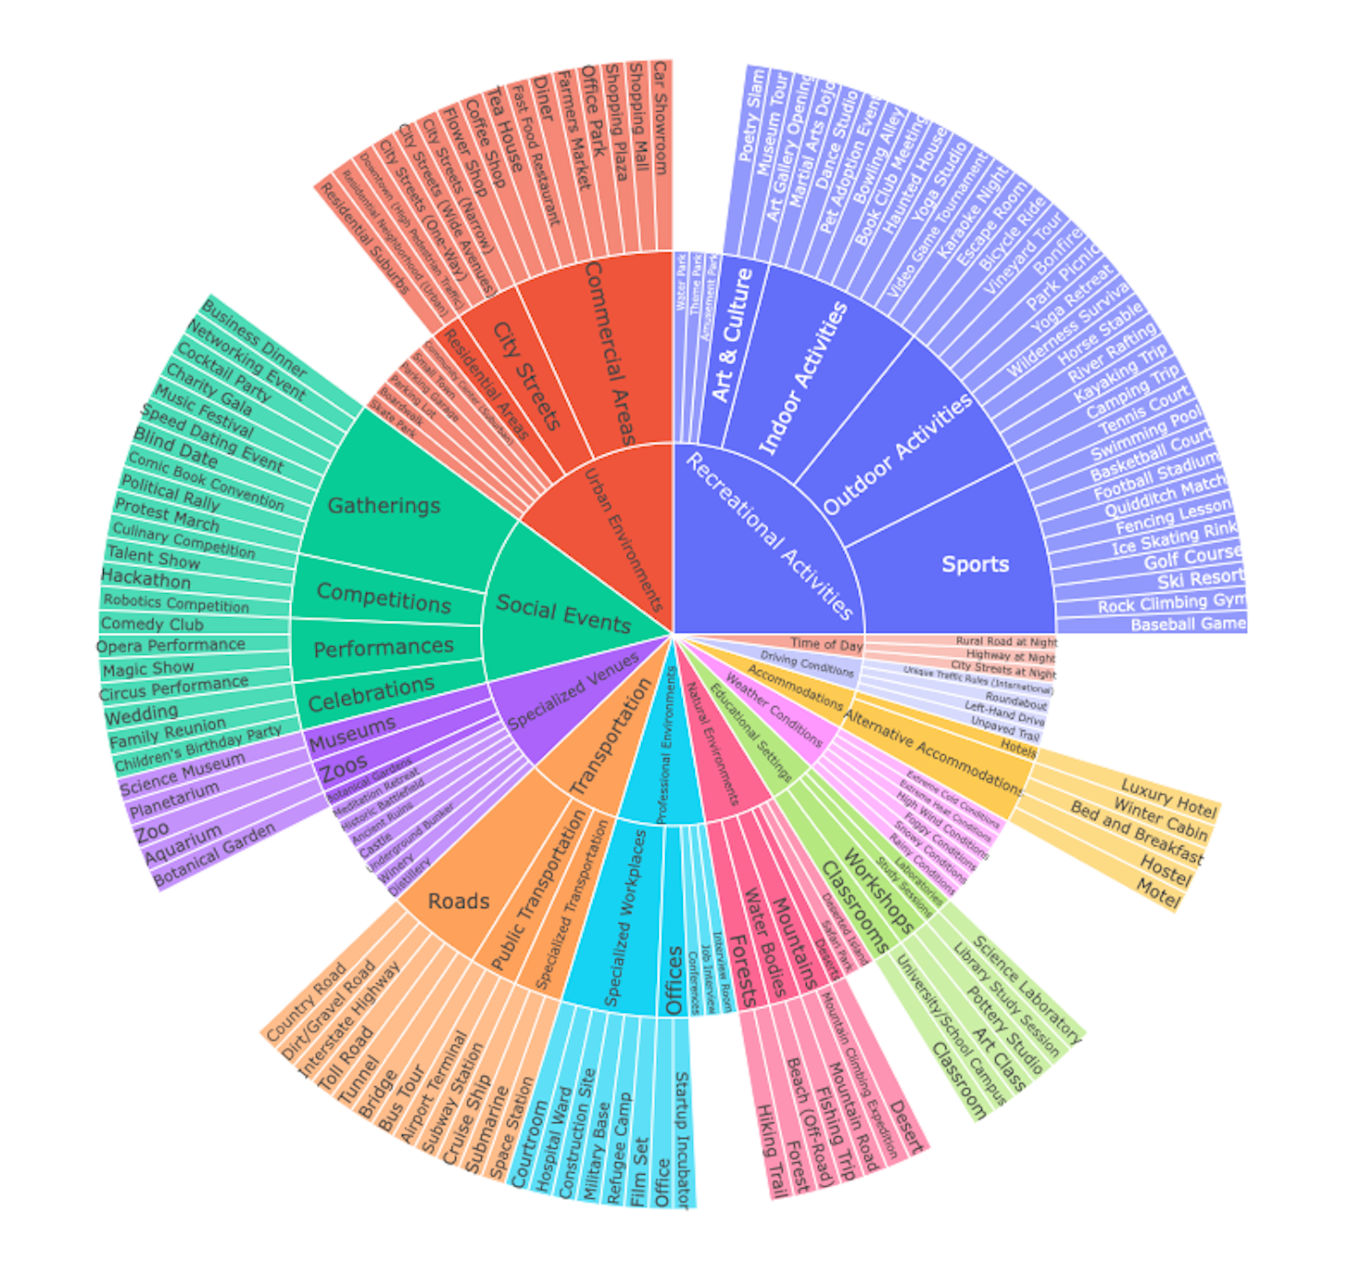
\includegraphics[width=8.3cm]{figures/environments-cropped.pdf}
         \vspace{1pt}
         \label{fig:visual_environment}
     \end{subfigure}
     \hfill
     \begin{subfigure}{\columnwidth}
         \centering
         
\includegraphics[width=\columnwidth]{figures/diversity_personas_2-compressed.pdf}
         \label{fig:visual_personas}
     \end{subfigure}
     \caption{(Top) distribution of static environments in \benchmark helping to visualize the diversity of environments from which relevant environments are selected for a given persona. (Bottom) distribution of attributes in personas used in experimentation. (Full-size versions are attached to our Appendix - Figure \ref{fig:environments_big}, \ref{fig:personas_big}. Examples of complete persona descriptions are also provided in Appendix D).}
% \ref{box:personas}
     \label{fig:visual_environment_personas}

\end{figure}

\paragraph{Claude 3 Resistant to Role Playing}
Our experiments show \textsc{Claude 3 Haiku} strongly resists persona agent roles. Figure~\ref{fig:claude} demonstrates Claude's refusal rate for persona agent questions is 8.5 times higher than the second-highest model (\textsc{LLaMA-3-8b}) and 2.6 times greater than all other benchmarked models combined. Claude frequently cites its lack of ``personal experience'' and it being an ``AI Assistant'' as justification. This resistance likely stems from safety measures preventing harmful responses, as role-play can potentially bypass safety guardrails \cite{deshpande-etal-2023-toxicity}. Conversely, \textsc{Claude 3.5 Sonnet} shows robust performance without such resistance, raising questions about its safety restrictions compared to Claude 3 Haiku. Future work should investigate how \textsc{Claude 3.5 Sonnet} balances persona agent capabilities with safety considerations. 
\begin{figure}[]
\centering
 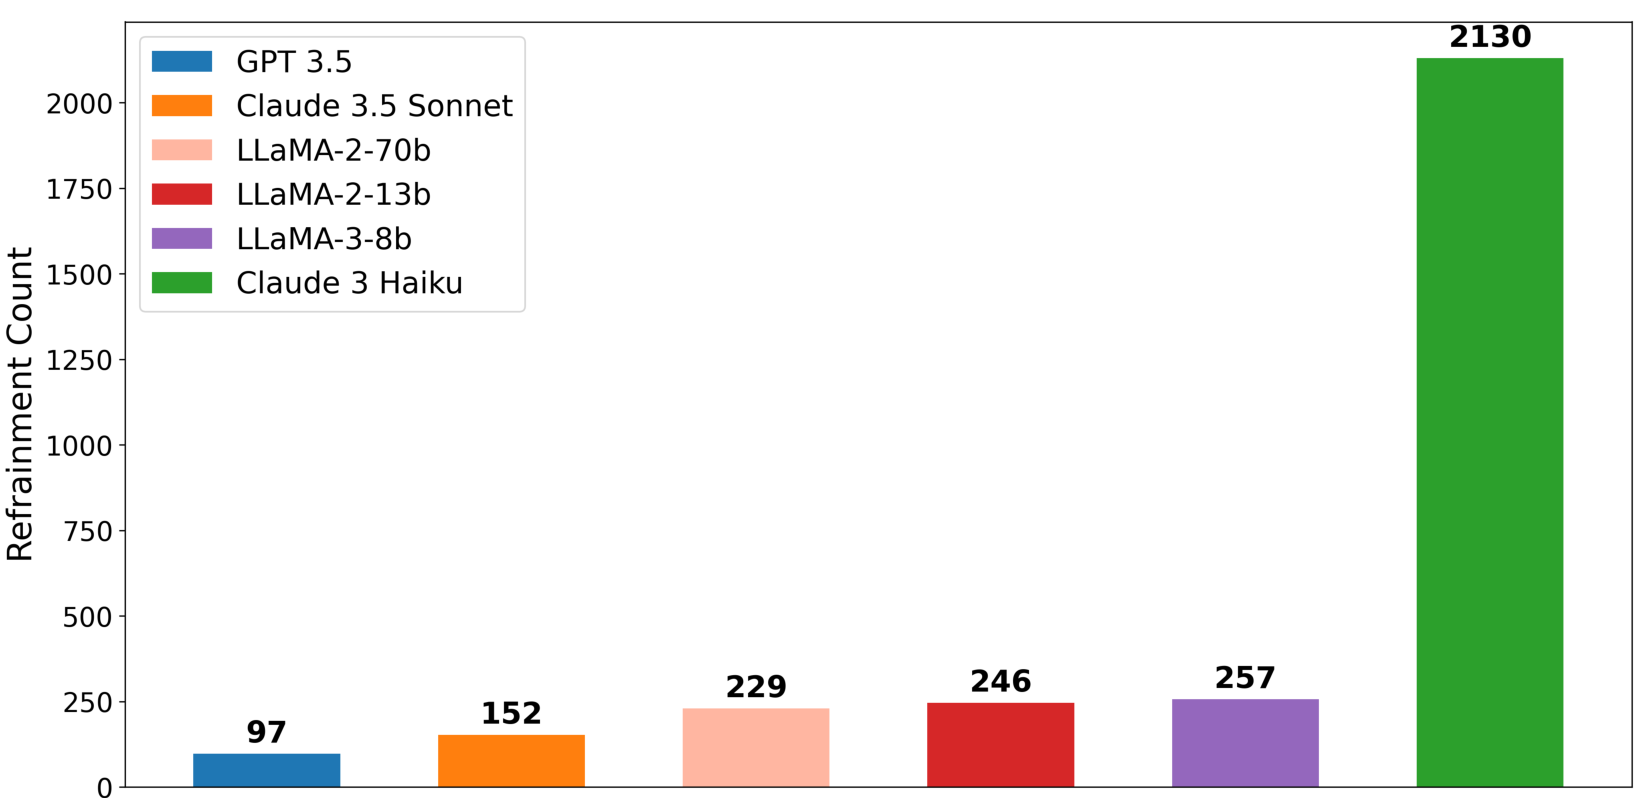
\includegraphics[width=\columnwidth]{figures/refrainment_counts.pdf}
 \caption{The number of refusals given role-play requests by LLMs. \textsc{Claude 3 Haiku} is strongly opposed to role-play instructions.}
 \label{fig:claude}

\end{figure}

\subsection{\benchmark is robust to model bias}
\label{sec:overreliance}

\begin{figure}[!th]
    
\includegraphics[width=0.5\textwidth]{figures/PersonaScore_comparison.pdf} 
    \caption{Cross-evaluation experiment of comparing performance across different question generator and evaluator model combinations for the same sample of 25 personas and environments.}
    \label{fig:robustness}
\end{figure}

In our pipeline, \textsc{GPT-4o} serves multiple functions (environment selection, question generation, and evaluation). To assess potential biases from using the same model across components, we conducted a robustness analysis similar to the cross-validation approach in \citet{judgebench}. We randomly sampled 25 personas from our benchmark of 200 and generated environments using \textsc{GPT-4o}. Questions were then generated using three different models (\textsc{GPT-4o}, \textsc{Deepseek-V3}, and \textsc{LLaMA-3.3-70b}), yielding 1,250 questions per generator. \textsc{GPT-4.1} served as the persona agent for answering all questions, with responses evaluated by multiple models (\textsc{Deepseek-V3}, \textsc{LLaMA-3.3-70b}, \textsc{GPT-4.5}, \textsc{GPT-4o}). Figure~\ref{fig:robustness} presents the \score results, showing no significant differences across question generators and evaluators, indicating minimal bias from using \textsc{GPT-4o} for both generation and evaluation. Additionally, circular evaluation bias was avoided as no evaluator model assessed responses from itself.

\subsection{Environments and Personas Distribution}
\benchmark encompasses diverse environments (Figure~\ref{fig:visual_environment_personas}), spanning social events ("Birthday Party," "Wedding"), recreational activities ("Hiking Trail," "Golf Course"), and gatherings ("Conference," "Hackathon"). The word cloud visualization reveals prominent persona attributes across professional roles ("teacher," "doctor"), locations ("New York," "Sydney"), and interests ("hiking," "advocating"), including specific traits like "vintage car enthusiast" and "environmental activist" suggesting that the experiments employ a wide spectrum of personas, enabling a thorough evaluation of LLMs' role-playing capabilities across different persona types and contexts.
